\documentclass{report}
\usepackage[T1]{fontenc}
\usepackage{color}
\usepackage{amssymb}
\usepackage{pdfpages}
\usepackage{amsmath}
\usepackage{eurosym}
\usepackage{graphicx}
\usepackage{textcomp}
\usepackage{listings}
\usepackage{epigraph}
\usepackage{longtable}
\usepackage{setspace}
\usepackage{array}
\usepackage{gensymb}
\usepackage{tikz}
\usepackage[some]{background}
\usepackage{geometry}
\usepackage[francais]{babel}


\begin{document}
\renewcommand{\chaptername}{Part}
\renewcommand{\thechapter}{\Roman{chapter}}

%\usepackage{lmodern}
%\usepackage{xspace}
%\usepackage{hyperref}

\definecolor{sup_strip_color}{rgb}{0.70,0.70,0.70}
\definecolor{inf_strip_color}{rgb}{0.00,0.00,0.00}

\DeclareFixedFont{\bigsf}{T1}{phv}{b}{n}{0.7cm}

\makeatletter                       
\def\printauthor{%                  
    {{\large \@author}}}              
\makeatother

\author{Zohour \textsc{Abouakil} ~\\ Sofia \textsc{Boutahar} ~\\ David \textsc{Courtinot} ~\\ Xiaowen \textsc{Ji} ~\\ Fabien \textsc{Sauce}}

\begin{titlepage}

\newgeometry{left=1cm,right=4cm,bottom=0cm}
\begin{tikzpicture}[overlay,remember picture]
% the black stripe with the title
\node[
  fill=inf_strip_color,
  anchor=north west,
  text width=\paperwidth,
  text height=2cm,
  text depth=2cm,
  inner xsep=1cm,
  font=\color{white}\bigsf 
  ] 
 at ([yshift=-2.5cm]current page.north west) (blackrect) {Development plan - Version 2};
% the khaki stripe
\path[fill=sup_strip_color] 
  (blackrect.north west) rectangle ++(\paperwidth,2.5cm);
\end{tikzpicture}

\vspace*{4.5cm}

\noindent
\begin{minipage}{0.35\linewidth}
    \begin{flushright}
        \printauthor
    \end{flushright}
\end{minipage} \hspace{15pt}
%
\begin{minipage}{0.02\linewidth}
    \rule{1pt}{175pt}
\end{minipage} \hspace{-10pt}
%
\begin{minipage}{0.6\linewidth}
\vspace{5pt}
\newenvironment{test}{\begin{center}}{\end{center}}
\hspace{10pt}
\begin{minipage}{\linewidth} 
\textbf{Reference :} model-checking.dev-plan ~\\
January $29^{th}$ 2015
\end{minipage}
\end{minipage}

\vspace{8cm}
\begin{minipage}{0.20\linewidth}
    \begin{flushright}
       
        \begin{tabular}{ll}
	 \textit{Signatures} & \\
            & \textbf{Quality responsible :} \\
            & \textbf{Clients :} \\
        \end{tabular}
    \end{flushright}
\end{minipage}

\end{titlepage}
\restoregeometry
\tableofcontents
\newgeometry{left=2.1cm,right=2.1cm}
\chapter{Project description and objectives}

\section{Surroundings of the project}

\subsection{What is "Projet long" ?}

\paragraph{}
\hspace{4mm}\textnormal{To get our ENSEEIHT engineering diploma, we are required to take part in 
a project called "Projet long" in teams of five students to work 
on a common project.}

\paragraph{}
\hspace{4mm}\textnormal{The project started on January 19, and will last eight weeks. It ends up with 
a defense in which we promote our work in front of a jury which evaluates 
us against different aspects :}

\vspace{4mm}
\begin{itemize}
\item Project management and organization\vspace{1mm}
\item Technical accomplishment\vspace{1mm}
\item Report and defense presentation\vspace{1mm}
\item English evaluation\vspace{1mm}
\end{itemize}

\paragraph{}
\hspace{4mm}\textnormal{All over the project, we have to work side by side with the client
 for whom we have to deliver, at the end of the project,
 a product that suits their expectations. Furthermore, we are 
also supervised by Mr. Jean-Francois COIFFIN. He is in charge 
of helping us through his experience in the project management and 
organization.}

\subsection{Who are our clients ?}

\paragraph{}
\hspace{4mm}\textnormal{The subject that we work on was made by Mr. David Doose and
 Mr. Julien Brunel, two researchers at Aerospace Lab ONERA. They are
 working on robot development using C++ language. This is why they are
 in the need of a model checking tool to assert some properties on their 
embedded system's code. The client already has a similar product, called Coccinelle. 
However, Coccinelle is limited to looking for patterns in C code.}

\subsection{What made us choose this subject ?}

\paragraph{}
\hspace{4mm}\textnormal{We chose to work on that project because of the originality of the subject, since it is mixing theoretic computer science and technical advanced principles.
       Moreover, studying model checking and temporal logic to assert properties on a source code was a topic that we studied in ENSEEIHT courses. This project is an opportunity to apply this theory and dive deeper into it.}

\section{Project description}

\subsection{Main idea}

\paragraph{}
\hspace{4mm}\textnormal{The client is waiting for a prototype that allows a search of patterns on a C++ code. The patterns will be expressed in terms of temporal logic properties.}

\subsection{Project parts}

\paragraph{}
\hspace{4mm}\textnormal{The project can be divided into two main parts :}

\vspace{4mm}
\begin{itemize}
\item \textbf{Parser :} takes a C++ code file as an input and transforms it into a data structure -a graph called CFG, as in Control Flow Graph- to explore every possible execution trace\vspace{1mm}
\item \textbf{Model checking algorithm :} this algorithm takes a property to check and tries to find the nodes in the graph that verify it.\vspace{1mm}
\end{itemize}

\paragraph{}
\hspace{4mm}\textnormal{After realizing both parts separately, we have to make it work togetger : this is the final product.
The following graph shows the main steps in our project.}

\begin{center}
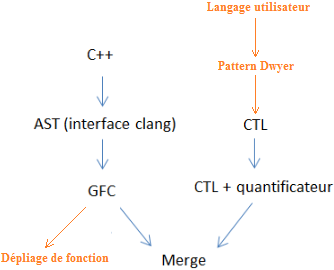
\includegraphics[scale=0.7]{data/tasks}
~\\~\\Figure I.1 - Project parts
\end{center}

\paragraph{}
\hspace{4mm}\textnormal{The tasks colored in orange represent possible (and optional) extensions of the product.}

\subsection{Related technologies}

\paragraph{}
\hspace{4mm}\textnormal{To simplify the C++ code parsing we will use an intermediate tool : Clang. It is a compiler front-end for C, C++, Objective-C and Objective-C++ and developed by Apple. It takes a C++ file as input and outputs a file describing an AST (Abstract Syntax Tree).}

\section{Final project}

\subsection{Functionalities}

\paragraph{}
\hspace{4mm}\textnormal{Features expected by the customer :}

\vspace{4mm}
\begin{itemize}
\item implementation of a parser for the AST generated by Clang\vspace{1mm}
\item a conversion from AST to a Scala model representation of the code in terms of graph
                control flux\vspace{1mm}
\item independently of the two preceding items , algorithms for the analysis of CTL properties (Computation Tree Logic) on some control flow graphs\vspace{1mm}
\item adding to the previous item some quantifiers such as "exists". This is known as CTL-V (CTL with quantified variables).\vspace{1mm}
\end{itemize}

\paragraph{}
\hspace{4mm}\textnormal{The following extensions can be added afterwards:}

\vspace{4mm}
\begin{itemize}
\item unfolding function calls on a given depth\vspace{1mm}
\item creating a user language to interface with the system\vspace{1mm}
\end{itemize}

\subsection{Deliverable documents and define priorities}

\paragraph{}
\hspace{4mm}\textnormal{Deliverables expected by the client are:}

\vspace{4mm}
\begin{itemize}
\item Documented source code in Scala language\vspace{1mm}
\item Test strategy\vspace{1mm}
\end{itemize}

\paragraph{}
\hspace{4mm}\textnormal{Deliverables expected by the supervisor and ENSEEIHT are:}

\vspace{4mm}
\begin{itemize}
\item Report in PDF format\vspace{1mm}
\item Development plan in PDF format\vspace{1mm}
\item Presentation supports\vspace{1mm}
\end{itemize}

\chapter{Project organization}

\section{Roles definition}

\subsubsection{Project manager}

\paragraph{}
\hspace{4mm}\textnormal{The project manager is primarily concerned about communications with the industrial and the customers. It has a leading role in the organization and planning of the tasks.}

\subsubsection{Supervisor}

\paragraph{}
\hspace{4mm}\textnormal{The supervisor has a global technical view of the project. He supervises the advancement of simultaneous tasks. Otherwise, he can rearrange groups and objectives if an unforeseen occurs. The supervisor has also to participate in coding or documenting an assigned task. Nevertheless, it is not his primary function.}

\paragraph{}
\hspace{4mm}\textnormal{The team supervisor can change from one week to another.}

\subsubsection{Quality manager}

\paragraph{}
\hspace{4mm}\textnormal{The quality manager is in charge of checking that every deliverable documents meets the quality standards. In other words, any produced code will pass under the watchful eye of the quality manager before being validated. He also ensures the quality and consistency of all documents produced by the team.}

\subsubsection{Test manager}

\paragraph{}
\hspace{4mm}\textnormal{The test manager is responsible of the validation and testing in global environment written by the developers (each developer has its own set of unit tests). He does not only run tests, he also determines whether the tests are complete or not (code coverage).}

\subsubsection{Configuration manager}

\paragraph{}
\hspace{4mm}\textnormal{The configuration manager should take care of every tool we are going to use, make some choice about which tools are better than other (example :
Scalastyle, an Eclipse plugin that we use for automated quality checs).
In particular he will handle the installation and the follow up of a version tool as Github for example.}

\subsubsection{Chain development}

\begin{center}
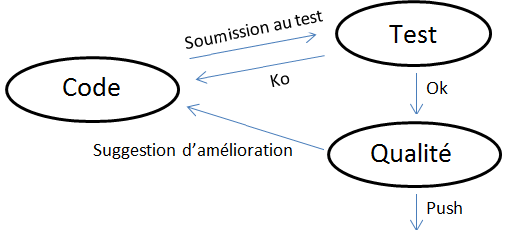
\includegraphics[scale=0.7]{data/cycle_qualite}
~\\~\\Figure II.1 - Sch\'{e}ma descriptif de la cha\^{i}ne de d\'{e}veloppement
\end{center}

\section{Development organisation}

\paragraph{}
\hspace{4mm}\textnormal{To secure our evolution we will use some methods inspired of famous project management techniques.}

\subsection{The Scrum method}

\paragraph{}
\hspace{4mm}\textnormal{We will try to use the Scrum method, which is widely used, and recognized for its effectiveness. At first, we will define a \textit{product backlog} containing all desired functionalities in the final product. In fact, this report is also a part of the \textit{product backlog}. 
Next, we will divide the project into three \textit{sprints} (which means iterations). A \textit{sprint backlog} is defined for each \textit{sprint}, including all we need to realise at the end of an iteration. Each \textit{sprint} lasts two weeks and lies in improve the software 
incrementally, so that it is close to \textit{product backlog}.}

\paragraph{}
\hspace{4mm}\textnormal{At the end of each \textit{sprint}, we will organise a meeting, in order to review the progress and propose improvements or modifications of planning,
 but in the process of a \textit{sprint}, we cannot modify the \textit{sprint backlog}. 
To finish, each day starts with a \textit{scrum meeting}, on the meeting, each 
team member present his objective of the day and his actual difficulties.}

\subsection{Team repartition approach}

\paragraph{}
\hspace{4mm}\textnormal{We will use an approach inspired by the XP (extreme programming) method. 
Considering the amount of code that we will have to write, we find it unnecessary that the five team members work separately, 
and we consider as excellent to work in pairs, in order to prevent errors and bias 
of the program structure, so that we can save times in testing and debugging. 
As a consequence, four of us will work in pairs and the last one works individually. The groups repartition
may change as the tasks are completed.}

\section{Tasks organisation}

\subsection{Tasks definition}

\paragraph{}
\hspace{4mm}\textnormal{Sprint 1 backlog:}

\vspace{4mm}
\begin{itemize}
\item AST parsing of procedure C++ code\vspace{1mm}
\item CFG conversion from parsed AST\vspace{1mm}
\item Model checking with simple properties\vspace{1mm}
\end{itemize}

\paragraph{}
\hspace{4mm}\textnormal{Sprint 2 backlog:}

\vspace{4mm}
\begin{itemize}
\item AST parsing of object oriented C++ code\vspace{1mm}
\item CFG conversion from parsed AST\vspace{1mm}
\item Model checking with simple criteria\vspace{1mm}
\end{itemize}

\paragraph{}
\hspace{4mm}\textnormal{Sprint 3 backlog:}

\vspace{4mm}
\begin{itemize}
\item Improved CFG conversion from parsed AST\vspace{1mm}
\item Model checking with complex criteria\vspace{1mm}
\end{itemize}

\subsection{Planning}

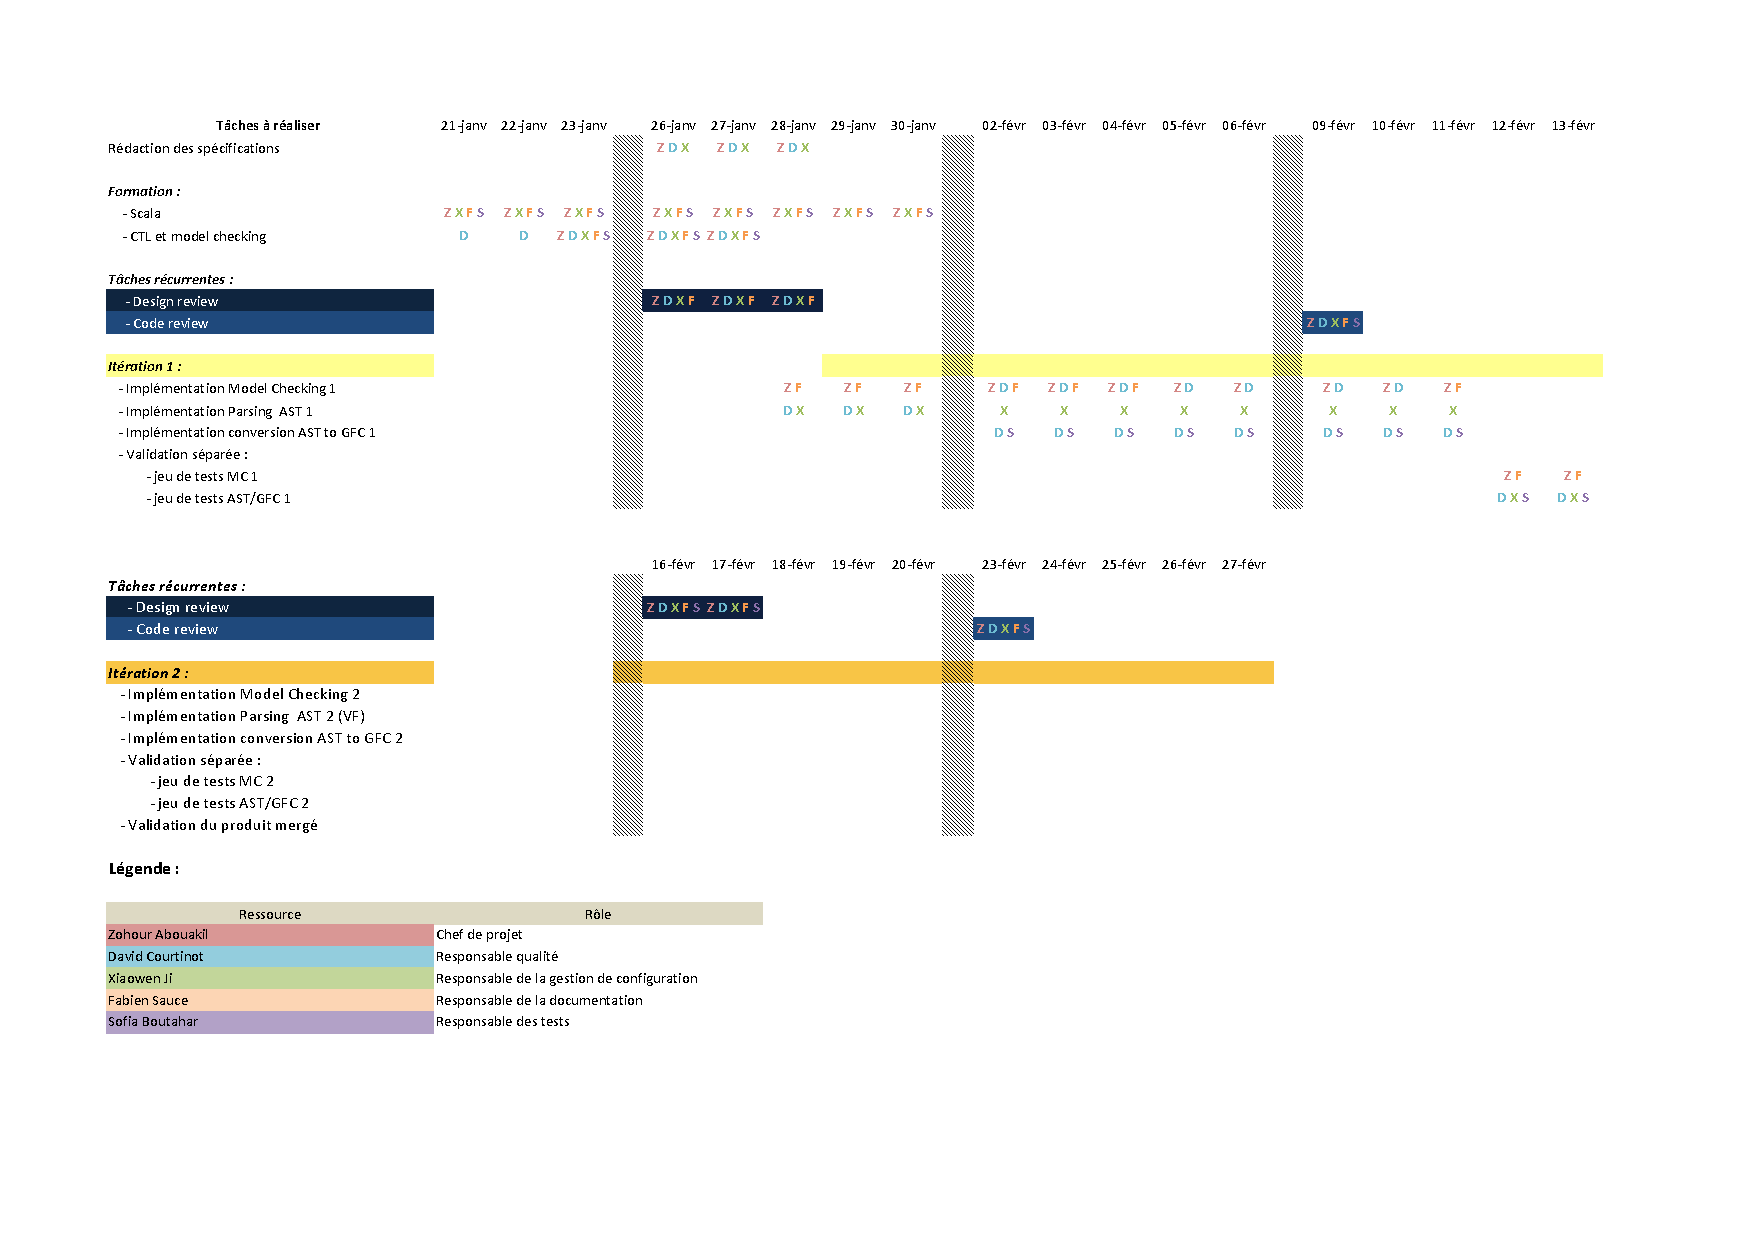
\includepdf[landscape=true,pages={1}]{data/planning.pdf}
\chapter{Risk management}

\paragraph{}
\hspace{4mm}\textnormal{}

%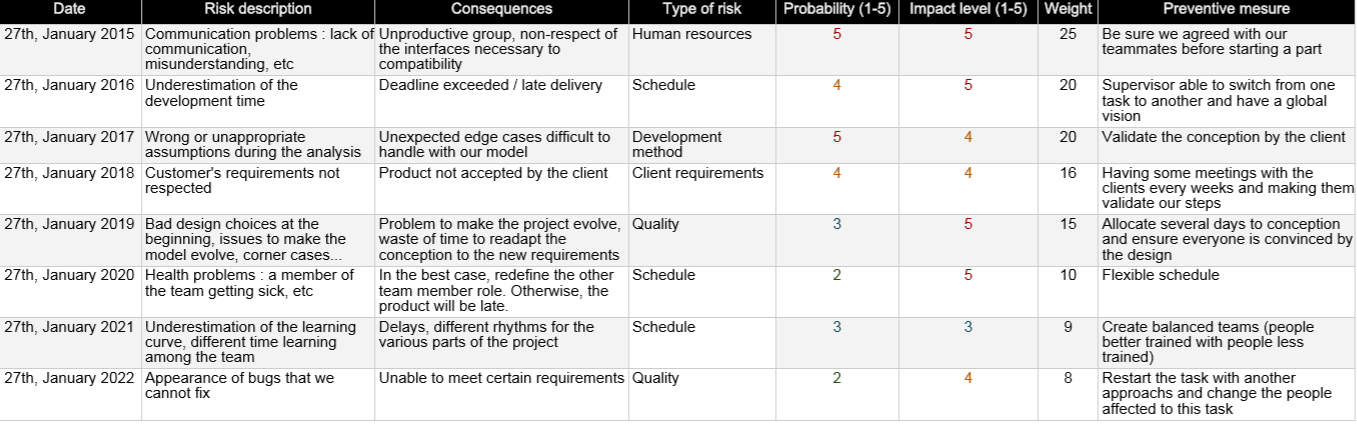
\includepdf[landscape=true,pages={1}]{data/risks.png}
%\newgeometry{left=1.5cm,,right=1.5cm}
\begin{center}
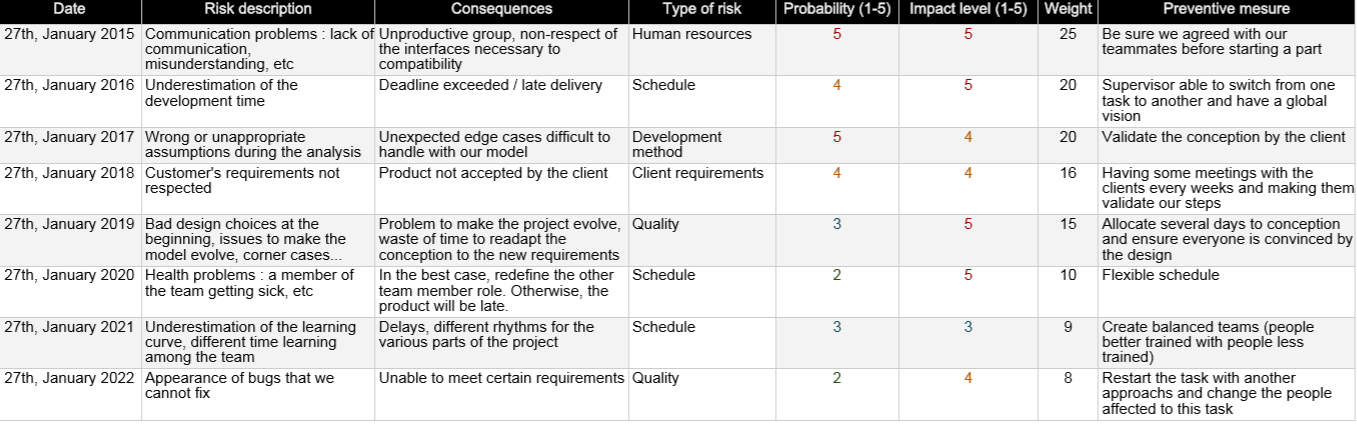
\includegraphics[scale=0.5]{data/risks.png}
~\\~\\Figure III.1 - Analyse des risques
\end{center}

\chapter{Code and documentation management}

\section{Quality management}

\subsection{Automated coding style checks}

\paragraph{}
\hspace{4mm}\textnormal{For ensuring that our coding rules are respected and evaluate the quality of our sources, we have
used a tool called \textit{Scalastyle} that enables, using an easy-to-use xml configuration file, to check
some properties on a Scala code. Combined with a specific pulgin, this can be use to generate warnings or errors
in the IDE the developer is using. Our settings are the following :}

%\newgeometry{left=1.5cm,,right=1.5cm}
\renewcommand{\arraystretch}{1.2}
\begin{center}
\begin{longtable}{|l|l|l|}
\hline
\textbf{Rule} & \textbf{Description} & \textbf{Value}  \\
\hline
FileLengthChecker & \small{Check the number of lines in a file} & 1500  \\
\hline
FileLineLengthChecker & \small{Check the number of characters in a line} & 140 \\
\hline
FileTabChecker & \small{Check that there are no tabs in a file} & enabled \\
\hline
ClassNamesChecker & \small{Check that class names match a regular}  & \^ [A-Z][A-a-z]*\$ \\
& \small{expression} & \\
\hline
\small{ClassTypeParameterChecker} & \small{Checks that type parameter to a class matches a} & \^[A-Z\_]\$ \\
& regular expression & \\
\hline
FileTabChecker & \small{Check that there are no tabs in a file} & enabled \\
\hline
\small{CyclomaticComplexityChecker} & \small{Checks that the cyclomatic complexity of a method} & 12 \\
&  \small{does exceed a value} & \\
\hline
EmptyClassChecker & \small{If a class/trait has no members, the braces are} & enabled \\
&  \small{unnecessary} & \\
\hline
\small{EqualsHashCodeChecker} & \small{Check that if a class implements either equals} & enabled \\ 
 & \small{or hashCode, it should implement the other} & \\
\hline
MagicNumberChecker & \small{Checks for use of magic numbers instead of} & ignore = -1, 0, 1 \\
& \small{constants (safer)} & \\
\hline
MethodLengthChecker & \small{Checks that methods do not exceed a maximum} & 50 \\
& \small{length} & \\
\hline
MethodNamesChecker & \small{Check that method names match a regular} & \^[a-z][A-Za-z0-9]*(\_=)?\$ \\
\tiny{.} & \small{expression} & \\
\hline
\small{MultipleStringLiteralsChecker} & \small{Checks that a string literal does not appear} & allowed = 2 \\
& \small{multiple times} & \\
\hline
\small{NotImplementedErrorUsage} & \small{Checks that the code does not have ??? operators} & enabled \\
\hline
NullChecker & \small{Check that null is not used} & enabled \\
\hline
\small{NumberOfMethodsInTypeChecker} & \small{Check that a class/trait/object does not have too} & maxMethods = 30 \\
& \small{many methods} & \\
\hline
NumberOfTypesChecker & \small{Checks that there are not too many types} & maxTypes = 20 \\
& \small{declared in a file} & \\
\hline
ObjectNamesChecker & \small{Check that object names match a regular}  & \^[A-Z][A-Za-z]*\$ \\
& \small{expression} & \\
\hline
ParameterNumberChecker & \small{Maximum number of parameters for a method} & maxParameters = 5 \\
\hline
RedundantIfChecker & \small{Checks that if expressions are not redundant, ie} & enabled \\
& \small{easily replaced by a variant of the condition} &  \\
\hline
ScalaDocChecker & \small{Checks that the ScalaDoc on documentable}  & enabled \\
& \small{members is well-formed} & \\
\hline
\end{longtable} 
\end{center}
% \restoregeometry
\renewcommand{\arraystretch}{1}
\subsection{Verification by pair}

\paragraph{}
\hspace{4mm}\textnormal{As we have opted for an XP model for the programming aspect of the project,
we consider that a code has passed the quality test if at least the two members of a pair
have checked it. This is up to the quality manager to ensure this has been done, otherwise he
should do it himself.}

\paragraph{}
\hspace{4mm}\textnormal{This is specific to the code quality checks and does not apply to the rest of the delivrable documents.}

\section{Test strategy}

\paragraph{}
\hspace{4mm}\textnormal{}

\section{Configuration management}

\paragraph{}
\hspace{4mm}\textnormal{All the delivrable documents are managed on a git repository, including documentation and reports.
Anyone is allowed to commit at anytime, however any push must have been authorized by the quality responsible after the code
has been thoroughly tested against a set of tests by the test responsible.}

\chapter{Appendices}

\end{document}
